\chapter{Optimal rational matrix function\\ approximation}
\label{chap:opt_algs}

We now shift gears a bit and consider methods for approximating \( \fA\vec{v} \) from Krylov subspace \( \mathcal{K}_k = \operatorname{span}\{\vec{v}, \vec{A}\vec{v}, \ldots, \vec{A}^{k-1}\vec{v} \} \).
The most ideal Krylov subspace method for this task would output iterates \( \mathsf{alg}_k \) satisfying
\begin{equation*}
    \mathsf{alg}_k = \argmin_{\vec{x}\in\mathcal{K}_k} \| \fA \vec{v} - \vec{x} \|.
\end{equation*}
The above condition guarantees the algorithm produces approximations with smaller error (in the given norm) than any other Krylov subspace method. 
Moreover, under the assumption \( \|\cdot\| \) is induced by a positive definite matrix with the same eigenvectors as \( \vec{A} \), \cref{thm:norm_exchange} implies the iterates satisfy a bound
\begin{equation*}
    \| \fA\vec{v} - \mathsf{alg}_k \| 
    \leq \min_{\deg(p) < k} \| \fA \vec{v} - \pA \vec{v} \|
    \leq \min_{\deg(p) < k} \| f - p \|_\Lambda \| \vec{v} \|.
\end{equation*}
In other words, the iterates satisfy a minimax bound \emph{on the eigenvalues of \( \vec{A} \)}.
As we saw in the introduction, a bound on the eigenvalues can be substantially stronger than a bound on an interval containing the eigenvalues.

A number of well-known algorithms, including the conjugate gradient (CG), minimum residual (MINRES), and quasi-minimum residual (QMR) algorithms, are standard methods for solving linear systems of equations $\vec{A}\vec{x} = \vec{v}$; i.e. for approximating $\vec{A}^{-1} \vec{v}$.
Each of these methods is \emph{optimal} for a certain norm and for certain classes of matrix \( \vec{A} \).
Moreover, such methods can be implemented in such a way that the amount of storage they use does not grow with the number of iterations \( k \). 

\iffalse
For general functions $f$ the situation is murkier. 
Presently, it is unknown whether general purpose KSMs, like the well-known Lanczos method for matrix function approximation (Lanczos-FA) \cite{saad_92}, which we discuss in \cref{chap:general_matfunc}, return near-optimal approximation to $\fA\vec{v}$ from $\mathcal{K}_k$, except in the case of particular functions such as the inverse or exponential \cite{druskin_greenbaum_knizhnerman_98}. 
% Instead, we must settle for weaker spectrum independent approximation guarantees \cite{musco_musco_sidford_18} \Chris{what's the right citation for these sorts of bounds?}. 
Work on more general spectrum dependent bounds remains somewhat ad-hoc, even for the basic case of rational functions \cite{eshof_frommer_lippert_schilling_van_der_vorst_02,ilic_turner_simpson_09,frommer_guttel_schweitzer_14,frommer_guttel_schweitzer_14a,chen_greenbaum_musco_musco_22a}.
Moreover, in terms of computational cost, to return an approximation to $\fA\vec{v}$ from $\mathcal{K}_k$ methods for general functions like Lanczos-FA require either (i) storing $k$ vectors of length $n$, or 
(ii) storing a constant number of vectors of length $n$, but increasing the number of matrix-vector products by a factor of two.
\fi

In this chapter, we describe the Lanczos method for optimal rational matrix function approximation (Lanczos-OR).
When $f$ is a rational function, Lanczos-OR outputs the \emph{optimal} (in a certain norm) approximation to $\fA\vec{v}$ from $\mathcal{K}_{k+1}$ using slightly more than $k$ matrix-vector products.
We provide a practical implementation of Lanczos-OR that
only requires storing a number of vectors of length $n$ proportional to the degree of the denominator in the rational function.
Therefore, for a fixed rational function, the storage costs do not grow with the iteration $k$. The approach used to derive this implementation of Lanczos-OR can also be used for computing the Lanczos-FA approximations to rational matrix functions, avoiding storage costs growing with $k$ in that widely used method.


Lanczos-OR is closely related to existing methods for linear systems. 
In particular, if $f = 1/(x-z)$, then, depending on the choice of $z$, the CG, MINRES, and QMR iterates can all be obtained as special cases of Lanczos-OR.
The Lanczos-OR iterate is mathematically equivalent to an optimal Galerkin projection method as described in \cite[Section 4]{lopez_simoncini_06}, provided the denominator matrix is positive definite. 
However, this method was mostly viewed as of theoretical interest since it could be used to help explain the behavior of Lanczos-FA. 
On the other hand, we show that such approximations can be computed efficiently.
Our approach is also somewhat more general in that it works with \emph{any} rational function.



\section{A bit of notation}


To simplify analysis, it will be useful to consider the recurrence that would obtained if the Lanczos algorithm were run to completion. 
In exact arithmetic, for some $K\leq n$, $\beta_{K-1} = 0$ in which case the algorithm terminates. 
Then, the final basis \( \Qhat := [ \vec{q}_0 , \ldots , \vec{q}_{K-1} ]\) and symmetric tridiagonal $\widehat{\vec{T}}$ with  diagonals $[\alpha_0, \ldots, \alpha_{K-1}]$ and off diagonals $[\beta_0, \ldots, \beta_{K-2}]$
satisfy
 a three-term recurrence 
\begin{equation}
    \label{eqn:lanczos_three_term_complete}
    \vec{A} \Qhat = \Qhat \widehat{\vec{T}}.
\end{equation}
%where \( \widehat{\vec{T}} \) is a real symmetric tridiagonal matrix with entries \Cam{I feel like we should move the picture up to where we first define $T$ and then just say what  $\hat T$ is without showing picture.} 
%\begin{equation*}
%    \widehat{\vec{T}}
 %   := \begin{bmatrix}
 %       \alpha_0 & \beta_0 \\
 %       \beta_0 & \alpha_1 & \ddots \\
 %       & \ddots & \ddots & \beta_{K-2}\\
 %       & & \beta_{K-2} & \alpha_{K-1}
 %   \end{bmatrix}.
%\end{equation*}
We emphasize that the algorithms we discuss \emph{do not} require Lanczos to be run to completion; the introduction of $\Qhat$ and $\widehat{\vec{T}}$ is for analysis purposes only.
% We often consider approximations from $\mathcal{K}_k$, and 
We note that $\vec{Q} = [\Qhat]_{:,:k}$ and $\vec{T} =[\widehat{\vec{T}}]_{:k,:k}$.
Since the columns of $\Qhat$ are orthogonal, we have that
\begin{equation*}
    \widehat{\vec{T}}
    = \Qhat^\cT \vec{A} \Qhat,
\end{equation*}
from which we easily see that, after any number of iterations $k$, $\vec{T} = \vec{Q}^\cT \vec{A} \vec{Q}$.
Note also that, for any shift $z\in\mathbb{C}$, 
\begin{equation*}
    (\vec{A} - z\vec{I}) \Qhat = \Qhat (\widehat{\vec{T}} - z\vec{I}).
\end{equation*}
In other words, the Krylov subspaces generated by $(\vec{A},\vec{v})$ and $(\vec{A}-z\vec{I},\vec{v})$ coincide, and the associated tridiagonal matrices are easily related by a diagonal shift. 
This shift invariance of Krylov subspaces is critical in a number of Krylov subspace methods.



\section{Existing algorithms}
\label{sec:linear_solvers}


It is well known that when $\vec{A}$ is positive definite, CG minimizes the $\vec{A}$-norm of the error over the Krylov subspace; i.e., the CG approximation $\mathsf{cg}_k$ is given by
\begin{equation*}
    \mathsf{cg}_k := \argmin_{\vec{x}\in\mathcal{K}_k}
    \| \vec{A}^{-1} \vec{v} - \vec{x} \|_{\vec{A}}.
\end{equation*}
%Recall that for a positive definite matrix $\vec{M}$, the norm $\|\vec{x}\|_{\vec{M}}$ denotes $\|\vec{x}\|_{\vec{M}} = \sqrt{\vec{x}^\cT\vec{M}\vec{x}}$. 
Since $\vec{Q}$ is a basis for $\mathcal{K}_k$, we can equivalently write
\label{eqn:cg_def}
\begin{equation*}
    \mathsf{cg}_k = \vec{Q} \argmin_{\vec{c}\in\R^k}
    \| \vec{A}^{1/2}(\vec{A}^{-1} \vec{v} - \vec{Q}\vec{c}) \|_2
    = \vec{Q} \argmin_{\vec{c}\in\R^k}
    \| \vec{A}^{-1/2} \vec{v} - \vec{A}^{1/2}\vec{Q}\vec{c} \|_2.
\end{equation*}
The solution to this least squares problem is
%Thus, by solving the normal equations \Anne{[This will be misleading to many people because it is the normal equations based on $\vec{A}^{1/2}$ not $A$.  Maybe just say ``The solution is ...''.]}, we arrive at the expression
\begin{equation*}
    \mathsf{cg}_k
    = \vec{Q} ( \vec{Q}^\cT \vec{A}^{1/2} \vec{A}^{1/2} \vec{Q})^{-1} \vec{Q}^\cT \vec{A}^{1/2} \vec{A}^{-1/2} \vec{v}
    = \vec{Q} \vec{T}^{-1} \vec{e}_0.
\end{equation*}
Here we have used that $\vec{Q}^\cT\vec{A}\vec{Q} = \vec{T}$ and that $\vec{Q}^\cT \vec{v} = \| \vec{v}\|_2\vec{e}_0 = \vec{e}_0$ (since we are assuming $\|\vec{v}\|_2=1$).

If $\vec{A}$ is indefinite, then the $\vec{A}$-norm of the error is not well defined and the CG iterates need not be optimal.
%\Anne{[This is not quite accurate since there is no norm defined analogously to the $A$-norm
%for positive definite $A$.  Maybe just omit this sentence?]}
A common alternative to CG for indefinite systems is MINRES, which minimizes the $\vec{A}^2$-norm of the error (the 2-norm of the residual) over the Krylov subspace; i.e., the MINRES approximation $\mathsf{mr}_k$ is given by
\begin{equation*}
    \mathsf{mr}_k
    := \argmin_{\vec{x}\in\mathcal{K}_k}
    \| \vec{A}^{-1} \vec{v} - \vec{x} \|_{\vec{A}^2}
    =
    \argmin_{\vec{x}\in\mathcal{K}_k}
    \| \vec{v} - \vec{A}\vec{x} \|_{2}
\end{equation*}
Now note that
\begin{equation*}
    \vec{A} \vec{Q} 
    = [\vec{A} \Qhat]_{:,:k}
    =[\Qhat\widehat{\vec{T}}]_{:,:k}
    =[\Qhat]_{:,:k+1} [\widehat{\vec{T}}]_{:k+1,:k}.
\end{equation*}
Therefore, since $\widehat{\vec{T}}$ is symmetric and $\Qhat$ has orthonormal columns,
%\begin{equation*}
%    \mathsf{mr}_k = \vec{Q} \argmin_{\vec{c}\in\R^k}
%    \| \vec{v} - \vec{A}\vec{Q} \vec{c} \|_{2}
%\end{equation*}
%so
\label{eqn:mr_def}
\begin{equation*}
    \mathsf{mr}_k = \vec{Q} (\vec{Q}^\cT \vec{A} \vec{A} \vec{Q})^{-1} \vec{Q}^\cT \vec{A} \vec{v}
    = \vec{Q} ([\widehat{\vec{T}}]_{:k,:k+1}[\widehat{\vec{T}}]_{:k+1,:k})^{-1} \vec{T} \vec{e}_0.
\end{equation*}

More generally,  suppose $z$ is an arbitrary complex number.
Then a special case of the quasi-minimum residual method (QMR) \cite{freund_92} can be used to compute the optimal $(\vec{A}^2+|z|^2 \vec{I})$-norm
approximation to $(\vec{A}-z \vec{I})^{-1}\vec{v}$; i.e., the QMR approximation $\mathsf{qmr}_k(z)$ is given by
\begin{align}
    \mathsf{qmr}_k(z)
    &:= \argmin_{\vec{x}\in\mathcal{K}_k}
    \| (\vec{A}-z \vec{I})^{-1} \vec{v} - \vec{x} \|_{(\vec{A}^2+|z|^2 \vec{I})}
    \nonumber\\&=
    \argmin_{\vec{x}\in\mathcal{K}_k}
    \| (\vec{A}-\overline z \vec{I})^{1/2}(\vec{A}-z \vec{I})^{-1/2}\vec{v} - (\vec{A}-\overline z \vec{I})^{1/2}(\vec{A}-z \vec{I})^{1/2}\vec{x} \|_{2}.
\end{align}
Here we have used that $\vec{A}^2+|z|^2 \vec{I} = (\vec{A}-\overline z \vec{I})(\vec{A}-z \vec{I})$.
Next, using the shift invariance of Krylov subspace, we see that
\label{eqn:qmr_def}
\begin{align*}
    \mathsf{qmr}_k(z)
    &:=  \vec{Q} (\vec{Q}^\cT (\vec{A}-\overline z \vec{I})(\vec{A}-z \vec{I}) \vec{Q})^{-1} \vec{Q}^\cT (\vec{A}- z \vec{I})\vec{v}.
    \\&=  \vec{Q} ( \vec{Q}( \vec{A}^2+|z|^2 \vec{I})\vec{Q}^\cT)^{-1} \vec{Q}^\cT (\vec{A}- \overline{z} \vec{I})\vec{v}
    \\&=  \vec{Q} ([\widehat{\vec{T}}]_{:k,:k+1}[\widehat{\vec{T}}]_{:k+1,:k}+|z|^2 \vec{I})^{-1} (\vec{T} - \overline{z} \vec{I})\vec{e}_0.
\end{align*}

%((\vec{A}-\Re(\theta)\vec{I})^2 + \Im(\theta)^2 \vec{I})

At first glance, CG, MINRES, and QMR all require the matrix \( \vec{Q} \) which is of size \( nk \).
However, by taking advantage of the tridiagonal structure of \( \widehat{\vec{T}} \), each of these algorithms can be implemented in a way which require storing just a few vectors of length $n$. 
In particular, the algorithms work by implicitly forming $\vec{L}\vec{D}\vec{L}^\cT$ factorization of \( \widehat{\vec{T}} \) \cite{paige_saunders_75,freund_92,liesen_strakos_13,simonova_tichy_21}.
The low-memory implementations for Lanczos-OR and Lanczos-FA that we derive in \cref{sec:low_mem} are based on this idea. 


\section{Optimal rational function approximation}


We now describe an optimal iterate for approximating $r(\vec{A})\vec{b}$ when $r$ is an arbitrary fixed rational function.
We will describe a low-memory implementation of this algorithm in \cref{sec:low_mem}.
Our low-memory implementation can also be used to compute the Lanczos-FA approximations to $r(\vec{A})\vec{b}$ without doubling the number of matrix-vector products.

\begin{definition}
\label{def:lanczos_or}
    Let \( r :\R\to\R \) be a rational function decomposed as \( r = M/N \), where \( N : \R\to\R \) is a polynomial with leading coefficient one and \( M:\R\to\R \) is a polynomial which does not divide \( N \).
For any polynomial \( R : \R\to\R \), define \( \tilde{M} = MR \) and \( \tilde{N} = NR \).
Then the Lanczos-OR iterate is defined as
\begin{equation*}
    \lanopt_k(r,R)
    :=  \vec{Q}  ([\tilde{N}(\widehat{\vec{T}})]_{:k,:k})^{-1} [\tilde{M}(\widehat{\vec{T}})]_{:k,:k} \vec{e}_0.
 \end{equation*}
\end{definition}

Those familiar with CG, MINRES, and the version of QMR for shifted Hermitian systems will note that these optimal algorithms are each obtained as special cases of Lanczos-OR.
Specifically, when $\vec{A}$ is positive definite, CG is obtained with \( r(x) = 1/x \) and \( R(x) = 1 \), MINRES is obtained with $r(x) = 1/x$ and \( R(x) = x \), and QMR is obtained if $r(x) = 1/(x-z)$ and \( R(x) = (x-\overline{z}) \).
In fact, we have a more general optimality result for Lanczos-OR:
\begin{theorem}
\label{thm:lanczos_opt}
    Given a rational function $r(x) = M(x)/N(x)$ as in \cref{def:lanczos_or}, choose a polynomial $R$ so that $\vec{H} = \tilde{N}(\vec{A}) = N(\vec{A})R(\vec{A})$ is positive definite.
Then $\lanopt_k(r,R)$ is the $\vec{H}$-norm optimal approximation to $r(\vec{A})\vec{v}$ from $\mathcal{K}_k$.
\end{theorem}


A simple way to ensure $\vec{H}$ is positive definite is to take \( R(x) = N(x) \) so that $\vec{H} = N(\vec{A})^2$.
However, in some situations, we may be able to get away with a lower degree choice for \( R \).
For instance, in the case of symmetric linear systems, while one can always use MINRES ($r(x)=1/xi$, $R(x)=x$), if \( \vec{A} \) is positive definite, then one may hope to use CG ($r(x)=1/x$, $R(x)=1$).
A simple way to obtain a lower degree choice of \( R \) is to only take the terms in \( N \) which are indefinite.
\begin{definition}
    \label{def:Rstar}
    Given a rational function $r = M/N$ as in \cref{def:lanczos_or}, factor 
    \begin{equation*}
        N(x) = \bigg( {\prod_{i=0}^{d_1-1}} (x-z_i) \bigg) \bigg( {\prod_{i=0}^{d_2-1}} (x-{z_i'})(x-\overline{z_i'}) \bigg)
    \end{equation*}
    where $z_i\neq \overline{z}_j$ for all $i,j = 0,1,\ldots, d_1-1$ with $j \neq i$.
    Then \( R^* \) is defined by
    \begin{equation*}
        R^*(x) = \xi {\prod_{i=0}^{d_1-1}} (x-\overline{z}_i)^{\alpha_i}   
    \end{equation*}    
    where, for \( i=0,1,\ldots,q-1 \), $\alpha_i = 0$ if $z_i\in \mathbb{R} \setminus \mathcal{I}$  and $\alpha_i = 1$ otherwise and $\xi \in \{ \pm 1 \}$ is chosen so that $R^*(\lambda_{\textup{min}})N(\lambda_{\textup{min}}) \geq 0$.  
\end{definition}

\begin{lemma}
    Given a rational function $r = M/N$ as in \cref{def:lanczos_or}, choose \( R^* \) as in \cref{def:Rstar}. 
    Then \( \vec{H} = N(\vec{A}) R^*(\vec{A}) \) is positive definite.
\end{lemma}

\begin{proof}
    Clearly $\prod_{i=0}^{q'-1} (x-{z'}_i)(x-\overline{z'}_i) \geq 0$ for all $x \in \mathbb{R}$, and for $z_i \in \mathbb{R} \setminus \mathcal{I}$, $(x-z_i)$ does not change signs over $\mathcal{I}$. 
The choice of $\xi$ ensures that $\tilde{N}(\lambda_{\textup{min}})>0$, and by assumption $N(\lambda) \neq 0$ for all $\lambda \in \Lambda$ so that that $\tilde{N}(\lambda) \neq 0$ for all $\lambda\in\Lambda$. 
It follows that $\tilde{N}(\lambda) > 0$ for all $\lambda\in\Lambda$; i.e. that $\vec{H} = \tilde{N}(\vec{A})$ is positive definite.
\end{proof}



\begin{proof}[Proof of \cref{thm:lanczos_opt}]
Since $\vec{y}\in\mathcal{K}_k$, we have $\vec{y} = \vec{Q} \vec{c}$ for some vector $\vec{c}$.
Thus, we can consider the problem
\begin{equation*}
    \argmin_{\vec{c}\in\R^k} \| r(\vec{A})\vec{v} - \vec{Q} \vec{c} \|_{\vec{H}}
    =
    \argmin_{\vec{c}\in\R^k} \| \vec{H}^{1/2} r(\vec{A})\vec{v} - \vec{H}^{1/2} \vec{Q} \vec{c} \|_2.
\end{equation*}
But this is just a standard least squares problem which has solution
\begin{equation*}
    \vec{c} = ( (\vec{H}^{1/2} \vec{Q})^\cT (\vec{H}^{1/2} \vec{Q}) )^{-1} (\vec{H}^{1/2} \vec{Q})^\cT (\vec{H}^{1/2} r\A \vec{v}).
\end{equation*}
Thus, we see that the optimal iterate has the form
\begin{equation*}
    \vec{Q}( \vec{Q}^\cT \vec{H} \vec{Q})^{-1} \vec{Q}^\cT \vec{H} r(\vec{A}) \vec{v}.
\end{equation*}
By definition, $\vec{H} = N(\vec{A})R(\vec{A}) $ so $\vec{H}r(\vec{A}) = M(\vec{A})R(\vec{A}) = \tilde{M}(\vec{A})$. Thus,
%By \cref{thm:lanczos_exact_poly}, if $k > \deg(\tilde{M})$, then
\begin{equation*}
    \vec{Q}^\cT \vec{H} r(\vec{A}) \vec{v}
    = \vec{Q}^\cT M(\vec{A}) \vec{v}
    = \vec{Q}^\cT \Qhat\tilde{M}(\widehat{\vec{T}}) \Qhat^\cT \vec{v}
    = [\tilde{M}(\widehat{\vec{T}})]_{:k,:k} \vec{e}_0.
\end{equation*}
Next, since $\vec Q$ consists of the first $k$ columns $\Qhat$,
\begin{equation*}
    \vec{Q}^\cT \vec{A}^q \vec{Q} = [\Qhat^\cT \vec{A}^q \Qhat]_{:k,:k}  
    % = (\widehat{\vec{I}}_k)^\cT \Qhat^\cT \vec{A}^q \Qhat \widehat{\vec{I}}_k
    % = (\widehat{\vec{I}}_k)^\cT  \widehat{\vec{T}}^q \widehat{\vec{I}}_k
    = [ \widehat{\vec{T}}^{q} ]_{:k,:k}
\end{equation*}
so since $\vec{H}$ is a linear combination of powers of $\vec{A}$ we obtain
\begin{equation*}
    \vec{Q}^\cT \vec{H} \vec{Q}
    = \vec{Q}^\cT \tilde{N}(\vec{A}) \vec{Q}
    =  [\tilde{N}(\widehat{\vec{T}}) ]_{:k,:k}.
\end{equation*}
The result follows by combining and rearranging the above expressions. 
\end{proof}

As we noted at the beginning of this chapter, the optimality of Lanczos-OR implies an a priori scalar polynomial error bound on the eigenvalues of $\vec{A}$ analogous to the well known minimax bounds for CG, MINRES, and QMR \cite{greenbaum_97}.
\begin{theorem}
Given a rational function $r = M/N$ as in \cref{def:lanczos_or} and a polynomial \( R \) so that $\vec{H} = \tilde{N}\A = N\A R\A$ is positive definite, 
\begin{equation*}
    \frac{\| r(\vec{A}) \vec{v} - \lanopt_k(r,R) \|_{\vec{H}}}{\| \vec{v} \|_{\vec{H}}}
    \leq \min_{\deg(p) < k} \max_{\lambda \in \Lambda} | r(\lambda) - p(\lambda) |.
\end{equation*}
\end{theorem}

\begin{proof}
Since $\lanopt_k(r,R)$ is the $\vec{H}$-norm optimal approximation over the Krylov subspace, we have
\begin{equation*}
    \| r(\vec{A})\vec{v} - \lanopt_k(r,R) \|_{\vec{H}}
    = \min_{\vec{x}\in \mathcal{K}_k} \| r(\vec{A})\vec{v} - \vec{x} \|_{\vec{H}}
    = \min_{\deg(p)<k} \| r(\vec{A})\vec{v} - p(\vec{A})\vec{v} \|_{\vec{H}}
\end{equation*}
Next, using the fact that $\vec{A}$ and $\vec{H}^{1/2}$ commute, we note that,
\begin{equation*}
    \| r(\vec{A})\vec{v} - p(\vec{A})\vec{v} \|_{\vec{H}}
    = \| (r(\vec{A})- p(\vec{A}))\vec{H}^{1/2}\vec{v} \|
    \leq \| r(\vec{A})- p(\vec{A}) \| \| \vec{v} \|_{\vec{H}}.
\end{equation*}
Finally, using the definition of the spectral norm,
\begin{equation*}
    \| r(\vec{A})- p(\vec{A}) \|
    = \| (r - p)(\vec{A}) \|
    = \max_{\lambda \in \Lambda} | r(\lambda)-p(\lambda) |.
\end{equation*}
The result follows.
\end{proof}


It is not yet apparent that the iterate can be computed efficiently. 
Indeed the expression involves the terms  $[\tilde{N}(\widehat{\vec{T}})]_{:k,:k}$ and $[\tilde{M}(\widehat{\vec{T}})]_{:k,:k}$, and computing $\widehat{\vec{T}}$ requires running Lanczos to completion.
However, since \( \widehat{T} \) is tridiagonal, these terms can be computed without much more information than is in $\vec{T}$ and the Lanczos-OR iterate can be computed with only a few more matrix vector products than required to compute the Lanczos-FA iterate.

\begin{lemma}
\label{thm:poly_That}
Suppose $p$ is a polynomial with $q := \deg(p) > 0$. 
Then $[p(\widehat{\vec{T}})]_{:k,:k}$ can be computed using the coefficients generated by $k+\lfloor (q-1)/2 \rfloor$ iterations of Lanczos.
Moreover, if $k':=k+\lfloor q/2 \rfloor$, then
\begin{equation*}
    [p(\widehat{\vec{T}})]_{:k,:k} = [p([\widehat{\vec{T}}]_{:k',:k'})]_{:k,:k}.
\end{equation*}
\end{lemma}

\begin{proof}
    Note that after \( k+d \) iterations of Lanczos, one obtains \( [\widehat{\vec{T}}]_{:k+d+1,:k+d} \).
    The result then follows immediately as a special case of \cref{thm:tridiag_power_dependence}.
\end{proof}

\iffalse
\begin{proof}%[Proof of \cref{thm:poly_That}]
It suffices to consider the case $p = x^q$.
Let $\widehat{\vec{I}}_\ell$ be the $K\times \ell$ matrix with the $\ell\times \ell$ identity in the top $\ell$ rows and zeros in the bottom $K-\ell$ rows.
Then, we have that 
\begin{equation*}
    \widehat{\vec{T}} \widehat{\vec{I}}_\ell
    = [\widehat{\vec{T}}]_{:,:\ell}
    = \widehat{\vec{I}}_{\ell+1} [\widehat{\vec{T}}]_{:\ell+1,:\ell}.
\end{equation*}
Repeatedly applying this relation,
\begin{equation*}
    \widehat{\vec{T}}^j \widehat{\vec{I}}_k
    = 
    \widehat{\vec{I}}_{k+j}
    [\widehat{\vec{T}}]_{:k+j,k+j-1}
    \cdots
    [\widehat{\vec{T}}]_{:k+2,k+1}
    [\widehat{\vec{T}}]_{:k+1,k}
    = \widehat{\vec{I}}_{k+j} \vec{B}(k+j,k)
\end{equation*}
where we have defined
\begin{equation*}
    \vec{B}(k+j,k) := [\widehat{\vec{T}}]_{:k+j,k+j-1}
    \cdots
    [\widehat{\vec{T}}]_{:k+2,k+1}
    [\widehat{\vec{T}}]_{:k+1,k}.
\end{equation*}
Therefore, since $(\widehat{\vec{I}}_{k+j})^\cT \widehat{\vec{I}}_{k+j}$ is the $(k+j)\times (k+j)$ identity,
\begin{equation*}
    [\widehat{\vec{T}}^{2j}]_{:k,:k}
    = \vec{B}(k+j,k)^\cT \vec{B}(k+j,k)
\end{equation*}
and, since $(\widehat{\vec{I}}_{k+j-1})^\cT \widehat{\vec{T}} \widehat{\vec{I}}_{k+j-1} = [\vec{T}]_{:k+j-1,:k+j-1}$,
\begin{equation*}
    [\widehat{\vec{T}}^{2j-1}]_{:k,:k}
    = \vec{B}(k+j-1,k)^\cT  [\widehat{\vec{T}}]_{:k+j-1,:k+j-1} \vec{B}(k+j-1,k).
\end{equation*}
In both cases, we see that these expressions depend only on $[\widehat{\vec{T}}]_{:k+j,:k+j-1}$ which can be obtained using $k+j-1$ matrix-vector products.
The result follows by noting that $\lfloor (2j-1)/2 \rfloor(x) = \lfloor(2j-1-1)/2 \rfloor(x) = j-1$.

To complete the lemma, note that for $\ell+1\leq k'$,
\begin{equation*}
    [\widehat{\vec{T}}]_{:k',:k'} \widetilde{\vec{I}}_\ell
    = [\widehat{\vec{T}}]_{:k',:\ell}
    = \widetilde{\vec{I}}_{\ell+1} [\widehat{\vec{T}}]_{:\ell+1,:\ell}
\end{equation*}
where $\widetilde{\vec{I}}_\ell$ is defined like $\widehat{\vec{I}}_\ell$ but is of size $k' \times \ell$.
The same argument as above then implies that
\begin{equation*}
    ([\widehat{\vec{T}}]_{:k',:k'})^j \widetilde{\vec{I}}_k
    =\widetilde{\vec{I}}_{k+j}\vec{B}(k+j,k)
\end{equation*}
provided that \( k+j \leq k' \).
We therefore have that
\begin{equation*}
    [\widehat{\vec{T}}^{q}]_{:k,:k} = [([\widehat{\vec{T}}]_{:k',:k'})^{q}]_{:k,:k}. 
\end{equation*}
\end{proof}
\fi

\subsection{Relation of Lanczos-OR to QMR on inverse quadratics}

The Lanczos-OR approximation to \( r(x) = 1/(x^2+|z|^2) \) is closely related to the approximation of two linear systems by QMR. 
\begin{lemma}
Suppose $z\in\R$ and define $r= 1/(x^2+|z|^2)$, $R^\pm = x\pm \ii z$, and $r^\pm = 1/R^\pm$.
Then, for all \( k\geq 1 \),
\begin{equation*}
    \lanopt_k(r,1)
    %= \frac{1}{2\ii z} \left( \lanopt_k(r^-,R^+) - \lanopt_k(r^+,R^-) \right).
    = \frac{1}{2\ii z} \left( \mathsf{qmr}_k(-\ii z) - \mathsf{qmr}_k(\ii z) \right).
\end{equation*}
\end{lemma}

\begin{proof}
Observe that
\begin{equation*}
    \lanopt_k(r^\pm,R^\mp) = \vec{Q}([\widehat{\vec{T}}^2+|z|^2\vec{I}]_{:k,:k})^{-1} [\vec{T} \mp \ii z \vec{I}]_{:k,:k} \vec{e}_0
\end{equation*}
so that 
\begin{equation*}
    \mathsf{qmr}_k(-\ii z) - \mathsf{qmr}_k(\ii z) 
    = 2 \ii z  \vec{Q}([\widehat{\vec{T}}^2+|z|^2\vec{I}]_{:k,:k})^{-1} \vec{e}_0
    = 2 \ii z \lanopt_k(r,1).
\end{equation*}
The result is then obtained by rearranging the above expression.
\end{proof}

Whether it is better to use Lanczos-OR with $r$ and $R=1$ or with $r^\pm$ and $R^\pm$ (i.e. QMR) is somewhat unclear.
The Lanczos-OR based approach avoids the need for complex arithmetic, which simplifies implementation slightly. 
However, since QMR has been studied longer, it is likely to have more practical low-memory implementations.


\section{Error estimates for Lanczos-OR}
\label{sec:error_OR}

We now describe an approach for estimating the Lanczos-OR error.
This approach has been widely studied for estimating the \( \vec{A} \)-norm of the error in CG, and we refer to \cite{strakos_tichy_02,meurant_tichy_18,estrin_orban_saunders_19,meurant_papez_tichy_21} and the references within for more details.
Note that several of these works also study whether such estimates are still reasonable in finite precision arithmetic as well as how to derive estimates for other norms such as the 2-norm.


\begin{theorem}
    \label{thm:OR_error}
Let \( r \) be a rational function and \( R \) a polynomial.
Write \( r(x) = M/N \) where \( N \) has leading coefficient one and \( M \) does not divide \( N \) and define \( \tilde{M} = MR \) and \( \tilde{N} = N R \).
Suppose \( \vec{H} = \tilde{N}\A \) is positive definite. 
Then the Lanczos-OR iterates satisfy,
\begin{equation*}
    \| r\A\vec{v} - \lanopt_k(r,R) \|_{\vec{H}}^2
    = \sum_{i=k}^{n-1}
    \| \lanopt_{i}(r,R) - \lanopt_{i+1}(r,R) \|_{\vec{H}}^2.
\end{equation*}

\end{theorem}

\begin{proof}
Let \( \{ \vec{p}_i \}_{i=0}^{n-1} \) be an \( \vec{H} \)-orthonormal set satisfying
\begin{equation*}
    \operatorname{span}\{\vec{p}_0, \ldots, \vec{p}_{i} \} 
    = \mathcal{K}_{i+1} 
\end{equation*}
for all \( i=0,1, \ldots, n-1 \), and decompose \( r\A\vec{v} \) as 
\begin{equation*}
    r\A\vec{v} = \sum_{i=0}^{n-1} c_i \vec{p}_i.
\end{equation*}
\Cref{thm:lanczos_opt} asserts that \( \lanopt_k(r,R) \) is the \( \vec{H} \)-norm optimal approximation to \( r\A\vec{v} \) from \( \mathcal{K}_k \).
Thus, for all \( j=0,1,\ldots, n-1 \), 
\begin{equation*}
    \lanopt_j(r,R) = \sum_{i=0}^{j-1} c_i \vec{p}_i.
\end{equation*}
This implies that
\begin{equation*}
    r\A\vec{v} - \lanopt_k(r,R) 
    = r\A\vec{v} - \sum_{i=0}^{k-1} c_i \vec{p}_i
    = \sum_{i=k}^{n-1} c_i \vec{p}_i.
\end{equation*}
    so that, by the \( \vec{H} \)-orthonormality of the \( \{ \vec{p}_i \}_{i=0}^{n-1} \),
\begin{equation*}
    \| r\A\vec{v} - \lanopt_k(r,R) \|_{\vec{H}}^2
    = \sum_{i=k}^{n-1} c_i^2.
\end{equation*}
    But we also have
    \begin{equation*}
        \lanopt_{i}(r,R) - \lanopt_{i+1}(r,R)
        = - c_i \vec{p}_i
    \end{equation*}
    so that
    \begin{equation*}
        \| \lanopt_{i}(r,R) - \lanopt_{i+1}(r,R) \|_{\vec{H}}^2 = c_i^2. \qedhere
    \end{equation*}
\end{proof}

Note that \cref{thm:OR_error} implies that
\begin{equation}
    \label{eqn:OR_est}
    \| r\A\vec{v} - \lanopt_k(r,R) \|_{\vec{H}}^2
    \geq \smop{\sum_{i=k}^{k+d-1}}
    \| \lanopt_{i}(r,R) - \lanopt_{i+1}(r,R) \|_{\vec{H}}^2.
\end{equation}
While this is a lower bound, if we assume that
\begin{equation*}
    \| r\A\vec{v} - \lanopt_{k+d}(r,R) \|_{\vec{H}}^2 = 
    \smop{\sum_{i=k+d}^{n-1}}
    \| \lanopt_{i}(r,R) - \lanopt_{i+1}(r,R) \|_{\vec{H}}^2
\end{equation*}
is negligible compared to \( \| r\A\vec{v} - \lanopt_k(r,R) \|_{\vec{H}}^2 \), then \cref{eqn:OR_est} becomes an approximate equality.

Typically $d$ can be taken as a small constant, say $d=5$, so the extra work required to obtain these estimate is not too large.

\begin{remark}
As shown in \cite{eshghi_reichel_21}, a similar approach can be used for general matrix functions. In particular, 
\begin{equation*}
    \| r\A\vec{v} - \mathsf{alg}_k \|
    \leq \| r\A\vec{v} - \mathsf{alg}_{k+d} \| + \| \mathsf{alg}_{k+d} - \mathsf{alg}_k \|
    \approx \| \mathsf{alg}_{k+d} - \mathsf{alg}_k \|
\end{equation*}
provided that \( \| r\A\vec{v} - \mathsf{alg}_{k+d} \| \ll \| r\A\vec{v} - \mathsf{alg}_k \| \).
    Note, however, that in situations where the convergence of \( \mathsf{alg}_k \) is oscillatory, it may be hard to guarantee \( \| r\A\vec{v} - \mathsf{alg}_{k+d} \| \ll \| r\A\vec{v} - \mathsf{alg}_k \| \), even if \( d \) is large.
\end{remark}



\subsection{Numerical experiment}

We choose \( \vec{A} \) with eigenvalues from the model problem \cref{eqn:model_problem} with \( n=300 \), \( \rho = 0.8 \), and \( \kappa = 1000 \) and \( \vec{b} \) with equal projection onto each eigencomponent.
We set \( r(x) = 1/(x^2+1) \), and run Lanczos-OR using \( R=1 \) with and without reorthgonalization.
In each case, we compute \cref{eqn:OR_est} with \( d=4 \).

The resulting estimates, shown in \cref{fig:ch5_OR_error_est}, are accurate for most iterations, with larger error in initial iterations where the true Lanczos-OR error is not decreasing as quickly as in later iterations.
Interestingly, the bound seems to work well in finite precision arithmetic.
Understanding this further is of interest.
In particular, a unified analysis of Lanczos-OR could provide more information about MINRES, for which existing bounds in finite precision arithmetic are somewhat weaker than CG.


\begin{figure}[htb]
    \begin{center}
        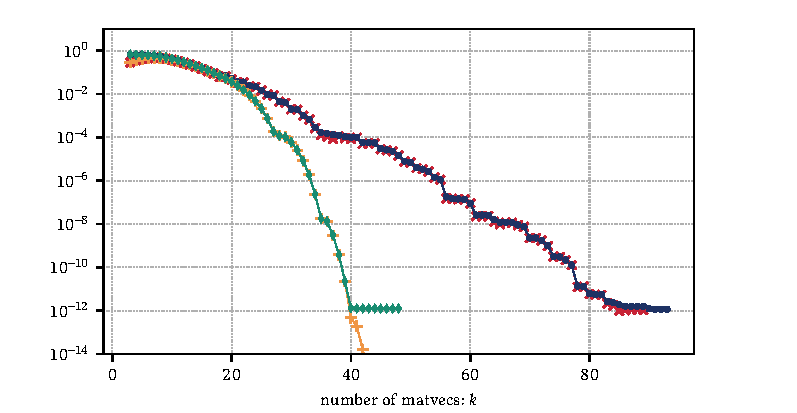
\includegraphics{imgs/ch5_OR_error_est.pdf} 
    \end{center}
    \caption[{Error estimates for Lanczos-OR for \( r(x) = 1/(x^2+1) \) and \( R(x) = 1 \).}]{%
    Error estimates for Lanczos-OR for \( r(x) = 1/(x^2+1) \) and \( R(x) = 1 \).
    \hspace{.25em}\emph{Legend}:
    Lanczos-OR error with reorthogonalization 
    ({\protect\raisebox{0mm}{\protect
\includegraphics[]{imgs/legend/l3.pdf}}}) 
    and corresponding estimate \cref{eqn:OR_est} with \( d=4 \)
    ({\protect\raisebox{0mm}{\protect
\includegraphics[]{imgs/legend/l4.pdf}}}).
    Lanczos-OR error without reorthogonalization 
    ({\protect\raisebox{0mm}{\protect
\includegraphics[]{imgs/legend/l1.pdf}}}) 
    and corresponding estimate \cref{eqn:OR_est} with \( d=4 \)
    ({\protect\raisebox{0mm}{\protect
\includegraphics[]{imgs/legend/l2.pdf}}}).
    \hspace{.25em}\emph{Takeaway}: The error estimates are remarkably accurate, even in finite precision arithmetic. 
    }
    \label{fig:ch5_OR_error_est}
\end{figure}



\section{Implementing Lanczos-OR using low memory}
\label{sec:low_mem}


We now describe a low-memory implementation of Lanczos-OR which is similar in spirit to CG, MINRES, and QMR. %In  particular, it is inspired by the LDL based version of CG described in \cite{simonova_tichy_21}.

For convenience, we will denote $\vec{M} := [\tilde{M}\mf{\widehat{\vec{T}}}]_{:k,:k}$ and $\vec{N} := [\tilde{N}\mf{\widehat{\vec{T}}}]_{:k,:k}$ so that the Lanczos-OR output is given by $\vec{Q} \vec{N}^{-1} \vec{M} \vec{e}_0$.
Then, at a high level, our approach is to:
\begin{itemize}
    \item Take one iteration of Lanczos to generate one more column of $\Qhat$ and $\widehat{\vec{T}}$
    \item Compute one more column of each of $\vec{M}$ and $\vec{N}$
    \item Compute one more factor of $\vec{L}^{-1} = \vec{L}_{k-1}\cdots \vec{L}_1 \vec{L}_0$ and one more entry of $\vec{D}$ where $\vec{L}$ and $\vec{D}$ are defined by the LDL factorization $\vec{N} =\vec{L}\vec{D}\vec{L}^\cT$
    \item Compute one more term of the sum:
    \begin{equation*}
        \vec{Q}\vec{N}^{-1}\vec{M}\vec{e}_0
        = \vec{Q} \vec{L}^{-1} \vec{D}^{-1} \vec{L}^{-\cT} \vec{M} \vec{e}_0 
        = \smop{\sum_{i=0}^{k-1}} \frac{[\vec{L}^{-\cT}\vec{M}\vec{e}_0]_i}{[\vec{D}]_{i,i}} [\vec{Q}\vec{L}^{-1}]_{:,i}
    \end{equation*}
\end{itemize}



There are two critical observations which must be made in order to see that this gives a memory-efficient implementation.
The first is that, since $\widehat{\vec{T}}$ is tridiagonal, $\vec{M}$, $\vec{N}$, and therefore $\vec{L}$ are all of half-bandwidth $q := \max(\deg(\tilde{M}),\deg(\tilde{N}))$.
This means that it is possible to compute the entries of $\vec{D}$ and the factors of $\vec{L}^{-1} = \vec{L}_{k-1}\cdots \vec{L}_1 \vec{L}_0$ one by one as we get the entries of $\widehat{\vec{T}}$.
The second is that because $\vec{L}$ is of bandwidth $q$, we can compute $[\vec{Q}\vec{L}^{-1}]_{:,i}$ without saving all of $\vec{Q}$. 
More specifically, $[\vec{L}^{-1} \vec{M} \vec{e}_0]_i$ and $[\vec{Q} \vec{L}^{-1}]_{:,i}$ can respectively be computed from $\vec{L}_{j-1}\cdots \vec{L}_1 \vec{L}_0 \vec{M} \vec{e}_0$ and $\vec{Q} \vec{L}_0^\cT \vec{L}_1^\cT \cdots \vec{L}_{k-1}^\cT$ and can therefore be maintained iteratively as the factors of $\vec{L}^{-1}$ are computed. 
Moreover, because of the banded structure of the factors $\vec{L}_i$, we need only maintain a sliding window of the columns of $\vec{Q}\vec{L}^{-1}$ which will allow us to access the relevant columns when we need them and discard them afterwards.

For clarity of exposition, we only describe how to compute $\vec{M}$ and $\vec{N}$ in the case that $\tilde{M}$ and $\tilde{N}$ are degree at most two.
The rest of the subroutines are fully described for any degree.
The syntax we use follows Python and other object oriented languages closely.

%, the intricacies of stably computing matrix polynomials in a manner compatible with our streaming approach, although interesting, is beyond the scope of this paper.
%This unlikely to be a major practical concern.
%Indeed, as we discussed in \cref{sec:rational_func}, when using a rational function obtained by discretizing an integral representation via a numerical quadrature, it is seemingly more natural to compute the term-wise optimal approximation.


\subsection{Computing LDL factorization}

For the time being, we will assume that we can sequentially access the rows of $\vec{M}$ and $\vec{N}$.
Our first step is to compute an LDL factorization of $\vec{N}$.
A LDL factorization can be computed via a symmetrized version of Gaussian elimination and is guaranteed to exist if \( \vec{N} \) is positive definite \cite{higham_02}.
Gaussian elimination can be viewed as transforming the starting matrix \( \vec{N}_0 = \vec{N} \) to a diagonal matrix \( \vec{N}_{k-1} = \vec{D} \) via a sequence of row and column operations
\begin{equation*}
    \vec{N}_{i+1} = \vec{L}_i \vec{N}_i \vec{L}_i^\cT
\end{equation*}
where
\begin{equation*}
    \vec{L}_i := 
    \vec{I}_k + \vec{l}_i\vec{e}_i^\cT
    ,\qquad
    \vec{l}_i := 
        \bigg[ \underbrace{\vphantom{\bigg|}0 , \cdots , 0}_{i+1\text{ zeros}} , -\frac{[\vec{N}_{i}]_{i+1,i}}{[\vec{N}_i]_{i,i}}  , \cdots , -\frac{[\vec{N}_i]_{k-1,i}}{[\vec{N}_i]_{i,i}}  \bigg]^\cT.
\end{equation*}
Note that the entries of \( \vec{L}_i \) are chosen to introduce zeros to the \( i \)-th row and column of \( \vec{N}_i \) such that \( [\vec{N}_{i+1}]_{:i+1,:i+1} \) is diagonal.
Therefore, if the algorithm terminates successfully, we will have obtained a factorization 
\begin{equation*}
    \vec{D} = (\vec{L}_{k-1} \cdots \vec{L}_1 \vec{L}_0) \vec{N} (\vec{L}_0^\cT \vec{L}_1^\cT \cdots \vec{L}_{n-1}^\cT)
\end{equation*}
where \( \vec{D} \) is diagonal and each \( \vec{L}_i \) is unit lower triangular.
To obtain the factorization \( \vec{N} = \vec{L} \vec{D} \vec{L}^\cT \), simply define  \( \vec{L} := (\vec{L}_{k-1} \cdots \vec{L}_1 \vec{L}_0)^{-1} \) and note that 
\begin{equation*}
    \vec{L} = \vec{I}_k - \smop{\sum_{i=0}^{k-1}} \vec{l}_i \vec{e}_i^\cT.
\end{equation*}
We remark that that $\vec{l}_{k-1}$ is the zeros vector and is only included in sums for ease of indexing later on. 
For further details on LDL factorizations, we refer readers to \cite{higham_02}.

To implement a LDL factorization, observe that the procedure above defines a recurrence
\begin{align*}
    [\vec{D}]_{j,j} &= [\vec{N}]_{j,j} - \smop{\sum_{\ell=0}^{j-1}} [\vec{L}_{j,\ell}]^2 [\vec{D}]_{\ell,\ell}
    \\
    [\vec{L}]_{i,j} &= \frac{1}{[\vec{D}]_{j,j}} \left( [\vec{N}]_{i,j} - \smop{\sum_{\ell=0}^{j-1}}[\vec{L}]_{j,\ell} [\vec{L}]_{i,\ell} [\vec{D}]_{\ell,\ell} \right)
    ,\qquad i > j.
\end{align*}
We therefore have \cref{alg:LDL}.

\begin{labelalgorithm}[htb]{LDL}{LDL}{LDL factorization}
\begin{algorithmic}[1]
    \Procedure{\thealgorithmname}{$\vec{N}$}
    \For{\(j=0,1,\ldots, k-1\)}
    \State \( [\vec{D}]_{j,j} = [\vec{N}]_{j,j} - \sum_{\ell=0}^{j-1} [\vec{L}_{j,\ell}]^2 [\vec{D}]_{\ell,\ell} \)
    \State \( [\vec{L}]_{j,j} = 1 \)
    \For{\(i=j+1, j+2, \ldots, k-1\)}
    \State \( [\vec{L}]_{i,j} = (1/[\vec{D}]_{j,j})( [\vec{N}]_{i,j} - \sum_{\ell=0}^{j-1}[\vec{L}]_{j,\ell} [\vec{L}]_{i,\ell} [\vec{D}]_{\ell,\ell} ) \)
    \EndFor
    \EndFor
    \State \Return \( \vec{L}, \vec{D} \)
\EndProcedure
\end{algorithmic}
\end{labelalgorithm}

\subsubsection{Streaming version}

%\Cref{thm:banded_LDL}
The fact that $\vec{L}$ has the same half bandwidth as $\vec{N}$ allows a more efficient implementation of \cref{alg:LDL} where terms which are known to be zero are not computed and only the important diagonals of $\vec{L}$ are stored.
Moreover, \cref{alg:LDL} already only accesses $\vec{N}$ one column at a time so it is easily converted to a streaming algorithm.
Making these changes gives the implementation \cref{alg:streaming_LDL} which is fed a stream of the columns of $\vec{N}$ in order, as shown in \cref{fig:streaming_LDL}.
Here the diagonal of $\vec{D}$ is stored as $\ms{d}$ and the $(j+1)$-st diagonal of $\vec{L}$ is stored as $[\ms{L}]_{j,:}$.
Thus, $\vec{L}_{i,j} = [\ms{L}]_{i-j-1,j}$ as long as $i-j \in 0:q+1$.


   
\begin{labelalgorithm}[htb]{streaming_LDL}{streaming-LDL}{Streaming LDL factorization}
\begin{algorithmic}[1]
\Class{\thealgorithmname}{$q,k$}
\State{stream: $[\vec{N}]_{0,0:q+1}, [\vec{N}]_{1,1:q+2}, \ldots, [\vec{N}]_{k-1,k-1:q+k-1}$}
\State $\ms{L} = \textsc{zeros}(q,k)$
\State $\ms{d} = \textsc{zeros}(k)$
\State $\ms{j}\gets0$
\Procedure{read-stream}{$\vec{n}$}
    \State $[\ms{d}]_{\ms{j}} \gets [\vec{n}]_0 - \sum_{\ell=\max(0,\ms{j}-q)}^{\ms{j}-1} [\ms{L}]_{\ms{j}-\ell-1,\ell}^2 [\ms{d}]_{\ell}$
%\State $[\ms{L}]_{0,\ms{j}} \gets 1$
    \For{$i=\ms{j}+1, \ms{j}+2, \ldots,  \min(\ms{j}-q,n-1)$}
    \State $[\ms{L}]_{i-\ms{j}-1,\ms{j}} \gets (1/[\ms{d}]_{\ms{j}})([\vec{n}]_{i-\ms{j}} - \sum_{\ell=\max(0,i-q)}^{i-1} [\ms{L}]_{i-\ell-1,\ell} [\ms{L}]_{\ms{j}-\ell-1,\ell} [\ms{d}]_{\ell} )$
\EndFor
\State $\ms{j}\gets \ms{j}+1$
\EndProcedure
\EndClass
\end{algorithmic}
\end{labelalgorithm}

\begin{figure}
    \centering
    \begin{subfigure}{.48\textwidth}\centering
    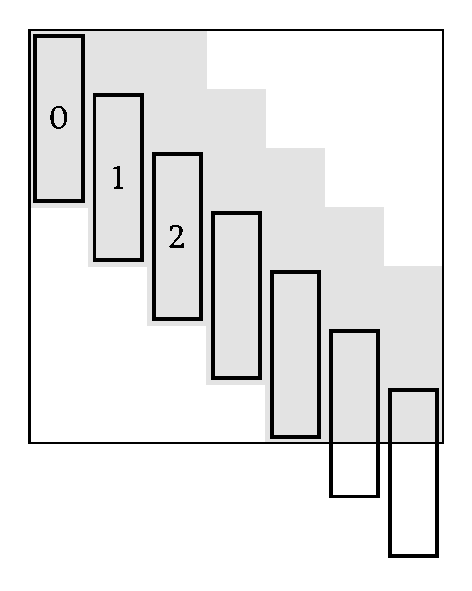
\includegraphics[height=4.5cm]{imgs/ch5_streaming_LDL.pdf}
    \caption{Pattern for $\vec{N}$ in \cref{alg:streaming_LDL}.}
    \label{fig:streaming_LDL}
    \end{subfigure}
    \hfill
    \begin{subfigure}{.48\textwidth}\centering
    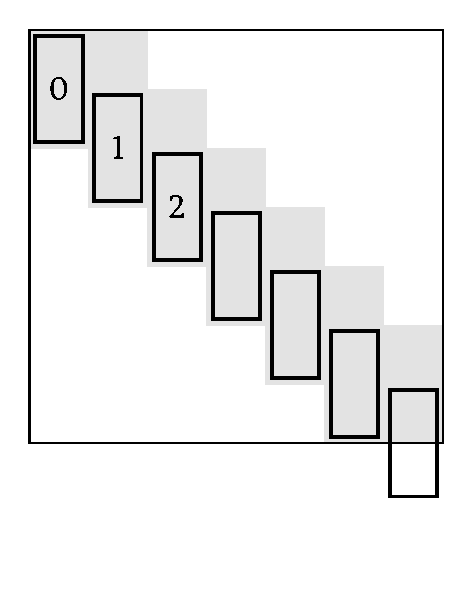
\includegraphics[height=4.5cm]{imgs/ch5_streaming_tridiag_square.pdf}
    \caption{Pattern for $\vec{T}$ in \cref{alg:streaming_tridiag_square}.}
    \label{fig:streaming_tridiag_square}
    \end{subfigure}
    \\
    \begin{subfigure}{\textwidth}\centering
    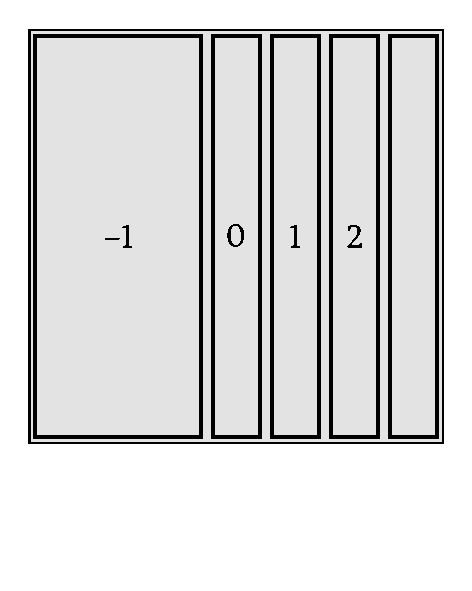
\includegraphics[height=4.5cm]{imgs/ch5_streaming_binv_Q.pdf}
    \hfill   
    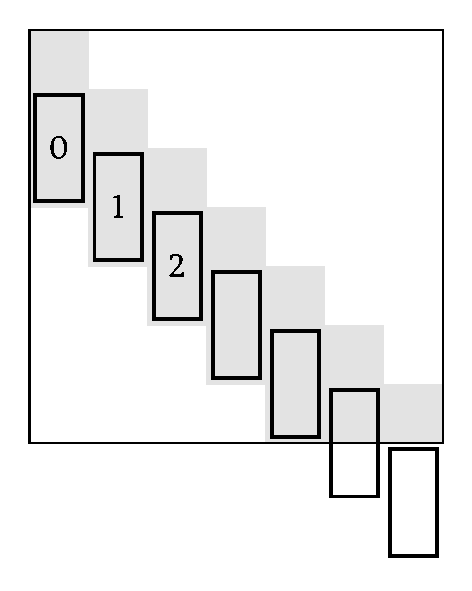
\includegraphics[height=4.5cm]{imgs/ch5_streaming_binv_L.pdf}
    \hfill    
    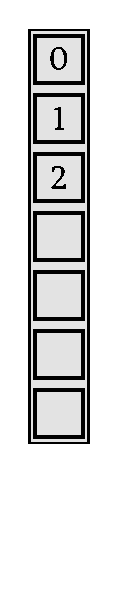
\includegraphics[height=4.5cm]{imgs/ch5_streaming_binv_d.pdf}
    \hfill
    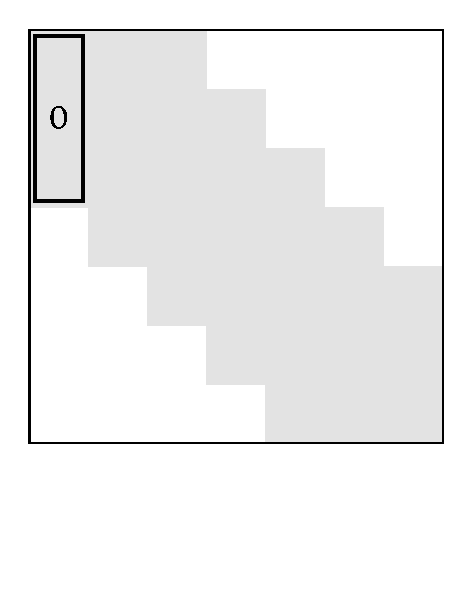
\includegraphics[height=4.5cm]{imgs/ch5_streaming_binv_M.pdf}
    \caption{Pattern for $\vec{Q}$, $\vec{L}$, $\vec{d}$, $\vec{M}$ in \cref{alg:streaming_banded_prod}.}
    \label{fig:streaming_banded_prod}
    \end{subfigure}
    \caption{Access patterns for inputs to streaming functions used in low-memory implementations of Lanczos-OR and Lanczos-FA.
    Indices indicate what information should be streamed into the algorithm at the given iteration.}
%    \label{}
\end{figure}


\begin{labelalgorithm}[htb]{streaming_banded_prod}{streaming-banded-prod}{Streaming banded product}
\begin{algorithmic}[1]
\Class{\thealgorithmname}{$n,k,q$}
\State{stream:$ $}
\State $\ms{X\_} \gets \textsc{zeros}(n,q+1)$
\State $\ms{y\_} \gets \textsc{zeros}(q+1)$
\State $\ms{out} \gets \textsc{zeros}(n)$
\State $\ms{j}\gets-1$
\Procedure{read-stream}{$\vec{v},\vec{l},d,\vec{y}_0$}
\If{$\ms{j}=-1$}
\State $[\ms{X\_}]_{:,:q} = \vec{v}$
\Else
\If{$\ms{i}=-1$}
\State $\ms{y\_} \gets \vec{y}_0$
\EndIf
\State $\ms{out} \gets \ms{out} + ([\ms{y\_}]_{0}/d)[\ms{X\_}]_{:,0}$
\State $[\ms{y\_}]_{:q} \gets [\ms{y\_}]_{1:} - [\ms{y\_}]_{0} \vec{l}$
\State $[\ms{y\_}]_{-1} \gets 0$
\State $[\ms{X\_}]_{:,-1} \gets \vec{v}$
\State $[\ms{X\_}]_{:,:q} \gets [\ms{X\_}]_{:,1:} + [\ms{X\_}]_{:,0} \vec{l}^\cT$
\EndIf
\State $\ms{j}\gets \ms{j}+1$
\EndProcedure
\EndClass
\end{algorithmic}
\end{labelalgorithm}


\subsection{Inverting the LDL factorization}

Once we have computed a a factorization \( \vec{N} = \vec{L}\vec{D}\vec{L}^\cT \), we can easily evaluate $\vec{Q}\vec{L}^{-1}\vec{D}^{-1} \vec{L}^{-\cT}\vec{M}\vec{e}_1$ using the fact that \( \vec{L}^{-1} = \vec{L}_{k-1} \cdots \vec{L}_1 \vec{L}_0 \).
Moreover, because the \( \vec{L}_j \) can be computed one at a time, there is hope that we can derive a memory efficient implementation.

Towards this end, define \( \vec{y}_j := \vec{L}_{j-1} \cdots \vec{L}_1 \vec{L}_0 \vec{M}\vec{e}_0 \) and \( \vec{X}_j := \vec{Q} \vec{L}_0^\cT \vec{L}_1^\cT \cdots \vec{L}_{j-1}^\cT  \).
Then, setting \( \vec{y}_{0} = \vec{M} \vec{e}_1 \) we have that
\begin{equation*}
    \vec{y}_{j+1} 
    = \vec{L}_{j} \vec{y}_{j}
    = (\vec{I} + \vec{l}_j \vec{e}_j^\cT ) \vec{y}_{j}
    = \vec{y}_{j} +  (\vec{e}_{j}^\cT \vec{y}_{j}) \vec{l}_j.
\end{equation*}
Similarly, setting \( \vec{X}_{0} = \vec{Q} \) we have that
\begin{equation*}
    \vec{X}_{j+1} 
    = \vec{X}_{j} \vec{L}_j^\cT
    = \vec{X}_{j} ( \vec{I} + \vec{e}_j \vec{l}_j^\cT)
    = \vec{X}_{j} + \vec{X}_{j} \vec{e}_j \vec{l}_j^\cT.
\end{equation*}
Then \( \vec{Q}\vec{L}^{-1}\vec{D}^{-1} \vec{L}^{-\cT}\vec{M}\vec{e}_1 = \vec{X}_{k} \vec{D}^{-1} \vec{y}_{k} \) can be computed accessing \( \vec{L} \), and therefore \( \vec{N} \), column by column.

\subsubsection{Streaming version}
\label{sec:streaming_banded_solve}

Recall that $[\vec{l}_i]_{:,\ell}$ is zero if $\ell \leq i$ or $\ell > i +q$.
Since $[\vec{l}_i]_{:i}$ is zero, we have
\begin{equation*}
    [\vec{y}_j]_j
    = [\vec{y}_{j} +  (\vec{e}_{j}^\cT \vec{y}_{j}) \vec{l}_j]_j
%    = [\vec{L}_j \vec{y}_j]_j
    = [\vec{y}_{j+1}]_j
    =\cdots
    = [\vec{y}_{k}]_j
\end{equation*}
and
\begin{equation*}
    [\vec{X}_{j}]_{:,j}
    = [\vec{X}_{j} + \vec{X}_{j} \vec{e}_j \vec{l}_j^\cT]_{:,j}
%    = [\vec{X}_{j}\vec{L}_j^\cT]_{:,j}
    = [\vec{X}_{j+1}]_{:,j}
    = \cdots = [\vec{X}_{k}]_{:,j}.
\end{equation*}
We therefore have that
\begin{equation*}
    \vec{X}_{k} \vec{D}^{-1} \vec{y}_{k}
    = \smop{\sum_{j=0}^{k-1}} \frac{[\vec{y}_{k}]_j}{[\vec{D}]_{j,j}} [\vec{X}_{k}]_{:,j}
    = \smop{\sum_{j=0}^{k-1}} \frac{[\vec{y}_{j}]_j}{[\vec{D}]_{j,j}} [\vec{X}_{j}]_{:,j}.
\end{equation*}
Similarly, since $[\vec{l}_i]_{i+q+1:}$ is zero,
\begin{equation*}
    [\vec{y}_j]_{j+q:}
    = [\vec{y}_{j-1} + (\vec{e}_{j-1}^\cT\vec{y}_{j-1}) \vec{l}_{j-1}]_{j+q:}
    = [\vec{y}_{j-1}]_{j+q:}
    = \cdots
    = [\vec{y}_0]_{j+q:}
\end{equation*}
and
\begin{equation*}
    [\vec{X}_{j}]_{:,j+q:}
    = [\vec{X}_{j-1}+\vec{X}_{j-1}\vec{e}_{j-1}\vec{l}_{j-1}^\cT]_{:,j+q:}
    = [\vec{X}_{j-1}]_{:,j+q:}
    =\cdots
    = [\vec{X}_{0}]_{:,j+q:}.
\end{equation*}
By definition, $\vec{y}_0 = \vec{M}\vec{e}_0$ and $\vec{X}_0 = \vec{Q}$.
Thus, we see that it is not necessary to know the later columns of $\vec{X}_j$ immediately. 

We can define a streaming algorithm by maintaining only the relevant portions of the $\vec{X}_i$ and $\vec{y}_i$.
Towards this end, define the length \( q+1 \) vector \( \bar{\vec{y}}_j := [\vec{y}_j]_{j:j+q+1} \) the \( n\times (q+1) \) matrix \( \bar{\vec{X}}_j = [\vec{X}_j]_{:,j:j+q+1} \).
Using the above observations, we see that these quantities can be maintained by the recurrences
\begin{equation*}
    \bar{\vec{y}}_j =  
    \begin{bmatrix}
        [\bar{\vec{y}}_{j-1}]_{1:}\\0
    \end{bmatrix}
    +  [\bar{\vec{y}}_{j-1}]_0 [\vec{l}_j]_{j+1:j+q+1} 
\end{equation*}
and
\begin{equation*}
    [\bar{\vec{X}}_j]_{:,:q}
    = [\bar{\vec{X}}_{j-1}]_{:,1:} 
        + ( [\bar{\vec{X}}_{j-1}]_{:,1} ) ([\vec{l}_j]_{j+1:j+q+1})^\cT
    ,\qquad
    [\bar{\vec{X}}_j]_{:,q} = [\vec{Q}]_{j+q}.
\end{equation*}
Note then that,
\begin{equation*}
    \vec{X}_{k-1} \vec{D}^{-1} \vec{y}_{k-1}
    = \smop{\sum_{j=0}^{k-1}}  \frac{[\bar{\vec{y}}_j]_{1}}{[\vec{D}]_{j+1,j+1}} [\bar{\vec{X}}_j]_{:,1}.
\end{equation*}

This results in \cref{alg:streaming_banded_prod} whose streaming pattern is outlined in \cref{fig:streaming_banded_prod}.


\begin{labelalgorithm}[htb]{streaming_banded_inv}{streaming-banded-inv}{Streaming banded inverse}
\begin{algorithmic}[1]
\Class{\thealgorithmname}{$n,k,q$}
\State{stream:$ $}
\State $\ms{LDL} \gets \textsc{streaming-LDL}(k,q)$
\State $\ms{Q0} \gets \textsc{zeros}(n,q)$
\State $\ms{j}\gets0$
\Procedure{read-stream}{$\vec{q},\vec{n},\vec{y}_0$}
\If{$\ms{j}<q$}
\State $[\ms{Q0}]_{:,j} \gets \vec{v}$
\If{$\ms{j}=q-1$}
    \State $\ms{b-prod} \gets \textsc{streaming-banded-prod}(n,k,q)$
    \State $\ms{b-prod.}\textsc{read-stream}(\ms{V0},\ms{none},\ms{none},\ms{none})$
\EndIf
\Else
\State $\ms{LDL.}\textsc{read-stream}(\vec{n})$
\State $\ms{b-inv.}\textsc{read-stream}(\vec{q},-[\ms{LDL.}\ms{L}]_{:,j-q},[\ms{LDL.}\ms{d}]_{j-q},\vec{y}_0)$
\EndIf
\State $\ms{j}\gets \ms{j}+1$
\EndProcedure
\EndClass
\end{algorithmic}
\end{labelalgorithm}



\subsection{Computing polynomials in $\vec{T}$}

The last major remaining piece is to construct $\vec{M} = \tilde{M}\mf{\vec{T}}$ and $\vec{N} = [\tilde{N}\mf{\widehat{\vec{T}}}]_{:k,:k}$.
Recall that we have assumed $\tilde{M}$ and $\tilde{N}$ are of degree at most two for convenience.
In iteration $\ell$ of Lanczos, we obtain $\alpha_{\ell}$ and $\beta_{\ell}$.
Observe that $\vec{T}^2$ is symmetric and that, defining $\beta_{-1} = \beta_{k} = 0$, the lower triangle is given by
\begin{equation*}
    [\vec{T}^2]_{i,j}
    = 
    \begin{cases}
    \beta_{j-1}^2 + \alpha_j^2 + \beta_j^2 & j=i \\
    (\alpha_j + \alpha_{j+1}) \beta_i & j=i-1 \\
    \beta_j \beta_{j+1} & j = i-2 \\ 
    0 & \text{o.w.}
    \end{cases}
\end{equation*}
%Thus, assuming we have stored $\{ \alpha_i \}_{i=1}^{\ell-1}$ and $\{ \beta_i \}_{i=1}^{\ell-1}$ we can compute $[\vec{M}]_{:\ell-1,:\ell-1}$ and $[\vec{N}]_{:\ell-1,:\ell-1}$.



We can use this to implement the streaming algorithm, \cref{alg:streaming_tridiag_square}, for computing the entries of $\vec{T}^2$.
Rather than being fed the entire tridiagonal matrix $\vec{T}$, \cref{alg:streaming_tridiag_square} is fed a stream of the columns of $\vec{T}$ in order, as shown in \cref{fig:streaming_tridiag_square}.
The algorithm respectively stores the $j$-th diagonals of $\vec{T}$ and $\vec{T}^2$  as $[\ms{T}]_{j,:}$ and $[\ms{Tp2}]_{j,:}$.

\begin{labelalgorithm}[htb]{streaming_tridiag_square}{streaming-tridiag-square}{Streaming tridiagonal square}
\begin{algorithmic}[1]
\Class{\thealgorithmname}{$k$}
\State{stream: $(\alpha_0, \beta_0), \ldots, (\alpha_{k-1},\beta_{k-1})$}
\State $\ms{T} \gets \textsc{zeros}(2,k)$
\State $\ms{Tp2} \gets \textsc{zeros}(3,k)$
\State $\ms{j}\gets0$
\Procedure{read-stream}{$\alpha,\beta$}
\State $[\ms{T}]_{0,\ms{j}} = \alpha$
\State $[\ms{T}]_{1,\ms{j}} = \beta$
\If{$\ms{i}=0$}
\State $[\ms{Tp2}]_{0,\ms{j}} \gets [\ms{T}]_{0,\ms{j}}^2+[\ms{T}]_{1,\ms{j}}^2$
\Else
\State $[\ms{Tp2}]_{0,\ms{j}} \gets [\ms{T}]_{0,\ms{j}}^2+[\ms{T}]_{1,\ms{j}}^2+[\ms{T}]_{1,\ms{j}-1}^2$
\State $[\ms{Tp2}]_{1,\ms{j}} \gets ([\ms{T}]_{0,\ms{j}}+[\ms{T}]_{0,\ms{j}-1})[\ms{T}]_{1,\ms{j}-1}$
\State $[\ms{Tp2}]_{2,\ms{j}} \gets [\ms{T}]_{1,\ms{j}}[\ms{T}]_{1,\ms{j}-1}$
\EndIf
\State $\ms{j}\gets \ms{j}+1$
\EndProcedure
\EndClass
\end{algorithmic}
\end{labelalgorithm}




Since we maintain the columns of $\vec{T}^2$ with \cref{alg:streaming_tridiag_square}, we can easily compute $\vec{M}$ and $\vec{N}$ using \cref{alg:get_poly}.

\begin{labelalgorithm}[htb]{get_poly}{get-poly}{Get polynomial of tridiagonal matrix}
\begin{algorithmic}[1]
\Procedure{\thealgorithmname}{$P,\ms{STp2},k,j$}
\State $a,b,c = P(0), P'(0), P''(0)$
\State $\vec{p} \gets \textsc{zeros}(3)$
\State $[\vec{p}]_{:3} \gets a [\ms{STp2.}\ms{Tp2}]_{:,j}$
\State $[\vec{p}]_{:2} \gets b [\ms{STp2.}\ms{T}]_{:,j}$
\State $[\vec{p}]_{:1} \gets c $
\EndProcedure
\end{algorithmic}
\end{labelalgorithm}

\subsection{Putting it all together}

With this algorithm in place, putting everything together is straightforward, and the full implementation is shown in \cref{alg:rational_lanczos}.

\begin{labelalgorithm}[htb]{rational_lanczos}{banded-rational}{Streaming banded rational inverse}
\begin{algorithmic}[1]
\Class{\thealgorithmname}{$n,k,\tilde{M},\tilde{N}$}
\State $\ms{b-inv} \gets \textsc{banded-inv}(n,k,2)$
\State $\ms{STp2} \gets \textsc{streaming-tridiag-square}(k)$
\State $\ms{j}\gets0$
\Procedure{read-stream}{$\vec{q},\alpha,\beta$}
\If{$\ms{j}<k$}
    \State $\ms{STp2.}\textsc{read-stream}(\alpha,\beta)$
    \State $\ms{b-inv.}\textsc{read-stream}($
    \State \hspace{1em} $\vec{q},$
    \State \hspace{1em} $\textsc{getpoly}(\tilde{N},\ms{STp2},k,\ms{j}-1)~\textbf{if}~\ms{j}\geq 2~\textbf{else}~\ms{none},$
    \State \hspace{1em} $\textsc{getpoly}(\tilde{M},\ms{STp2},k,\ms{j}-1)~\textbf{if}~\ms{j}= 2~\textbf{else}~\ms{none},$
    \State$)$
\EndIf
\State $\ms{LDL.}\textsc{read-stream}(\vec{n})$
\State $\ms{j}\gets \ms{j}+1$
\EndProcedure
\Procedure{finish-up}{$ $}
\For{$i=k,k+1$}
    \State $\ms{b-inv.}\textsc{read-stream}( \ms{none}, \textsc{getpoly}(\tilde{N},\ms{STp2},k,\ms{j}-1), \ms{none} )$
\EndFor
\EndProcedure
\Procedure{get-output}{$ $}
\State \Return \ms{b-inv.}\ms{b-prod.}\ms{out}
\EndProcedure
\EndClass 
\end{algorithmic}
\end{labelalgorithm}

This can be incorporated into any Lanczos implementation and used to compute the Lanczoz-OR iterates.
For concreteness, we show this with the implementation of Lanczos from \cref{alg:lanczos}.
We call the resulting implementation Lanczos-OR-lm.

\begin{labelalgorithm}[htb]{lanczos_OR}{Lanczos-OR-lm}{Lanczos-OR (low memory)}
\begin{algorithmic}[1]
\Procedure{\thealgorithmname}{$\vec{A},\vec{v},k,M,N$}
\State \( \vec{q}_{-1} = \vec{0} \),
\( \beta_{-1} = 0 \),
    \( \vec{q}_0  = \vec{v} \)
\State Set $\tilde{M}$ and $\tilde{N}$ as in \cref{def:lanczos_or}
\State $\ms{lam-lm} \gets \textsc{banded-rational}(n,k,\tilde{M},\tilde{N})$
\For {\( j=0,1,\ldots, k-1 \)}
    \State \( \tilde{\vec{q}}_{j+1} = \vec{A} \vec{q}_{j} - \beta_{j-1} \vec{q}_{j-1} \)
    \State \( \alpha_j = \langle \tilde{\vec{q}}_{j+1}, \vec{q}_j \rangle \)
    \State \( \tilde{\vec{q}}_{j+1} = \tilde{\vec{q}}_{j+1} - \alpha_j \vec{q}_j \)
%    \If{reorthogonalize}
        \State optionally, reorthogonalize \( \tilde{\vec{q}}_{j+1} \) against \( \{\vec{q}_i\}_{i=0}^{j-1} \)
%    \EndIf
    \State \( \beta_{j} = \| \tilde{\vec{q}}_{j+1} \| \)
    \State \( \vec{q}_{j+1} = \tilde{\vec{q}}_{j+1} / \beta_{j} \)
    %\If {Lanczos-FA-lm~\textbf{and}~$j=k-1$}
    %\State $\ms{lam-lm.}\textsc{read-stream}(\vec{q}_{k-1},\alpha_{k-1},0)$
    %\Else%If {Lanczos-OR-lm}
    \State $\ms{lam-lm.}\textsc{read-stream}(\vec{q}_{j},\alpha_{j},\beta_{j})$
    %\EndIf
\EndFor
\State $\ms{lam-lm.}\textsc{finish-up}()$
\EndProcedure 
\end{algorithmic}
\end{labelalgorithm}

We can easily obtain an implementation of Lanczos-FA, which we call Lanczos-FA-lm, by replacing $\beta_{k-1}$ with $0$ in the final iteration of the loop. 

\subsection{Some comments on implementation}

Our main goal is to describe how to implement Lanczos-FA and Lanczos-OR in a way that requires $k$ matrix-vector products and $O(n)$ storage, when $M$ and $N$ are each at most degree two. As mentioned, the approach can be extended to any constant degree.
There are a range of improvements to our implementation which may be useful in practice.

First, the amount of storage used can be reduced somewhat.
Indeed, the implementation described above saves $\vec{T}$, $\vec{T}^2$, $\vec{L}$, and $\vec{d}$, but only accesses a sliding window of these quantities.
We have chosen to save them for convenience since they require only $O(k)$ storage.
However, storing only the relevant information from these quantities would result in an implementation with storage costs independent of the number of iterations $k$.
In this vein, a practical implementation would likely determine $k$ adaptively by monitoring the residual or other measures of the error.
Improvements to the number of vectors of length $n$ may be possible as well.
For example, storage could possibly be reduced somewhat by incorporating the Lanczos iteration more explicitly with the inversion of the LDL facorization, much like the classical Hestenes and Stiefel implementation of CG \cite{hestenes_stiefel_52}.


As with other short-recurrence based Krylov subspace methods, the behavior of Lanczos-FA-lm and Lanzos-OR-lm in finite precision arithmetic may be different than in exact arithmetic.
However, with the exception of the Lanczos algorithm, the other aspects of our algorithm are essentially backwards stable.
It is therefore more or less clear that Lanczos-FA-lm and Lanczos-OR-lm will accurately compute the expressions $\vec{Q} N\mf{\vec{T}}^{-1} M\mf{\vec{T}} \vec{e}_0$ and $\vec{Q}  ([\tilde{N}\mf{\widehat{\vec{T}}}]_{:k,:k})^{-1} \tilde{M}\mf{\vec{T}} \vec{e}_0$ provided that $M\mf{\vec{T}}$ $N\mf{\vec{T}}$, $[\tilde{N}\mf{\widehat{\vec{T}}}]_{:k,:k}$ are reasonably well conditioned.
Indeed, in practice solving linear systems by symmetric Gaussian elimination is accurate; see for instance \cite[Chapter 10]{higham_02}.
Thus, such bounds and techniques can be applied to Lanczos-FA-lm and Lanczos-OR-lm.

\iffalse
However, our implementation is equivalent, even in finite precision arithmetic, to \begin{itemize}
    \item running Lanczos to obtain $\vec{Q}$ and $\vec{T}$
    \item computing $\vec{M}$ and $\vec{N}$ via certain standard approachs
    \item computing an LDL factorizaton of $\vec{N}$ via a certain standard approach
    \item computing $\vec{Q} \vec{L}^{-1} \vec{D}^{-1} \vec{L}^{-\cT}\vec{M}\vec{e}_0$ in an essentially standard way.
\end{itemize}
\fi


